\documentclass[11pt]{report}

% Paquetes y configuraciones adicionales
\usepackage{graphicx}
\usepackage[export]{adjustbox}
\usepackage{caption}
\usepackage{float}
\usepackage{titlesec}
\usepackage{geometry}
\usepackage[hidelinks]{hyperref}
\usepackage{titling}
\usepackage{titlesec}
\usepackage{parskip}
\usepackage{wasysym}
\usepackage{tikzsymbols}
\usepackage{fancyvrb}
\usepackage{xurl}
\usepackage{hyperref}
\usepackage{listings}
\usepackage{xcolor}
\usepackage[spanish]{babel}

\newcommand{\subtitle}[1]{
  \posttitle{
    \par\end{center}
    \begin{center}\large#1\end{center}
    \vskip0.5em}
}

% Configura los márgenes
\geometry{
  left=2cm,   % Ajusta este valor al margen izquierdo deseado
  right=2cm,  % Ajusta este valor al margen derecho deseado
  top=3cm,
  bottom=3cm,
}

% Configuración de los títulos de las secciones
\titlespacing{\section}{0pt}{\parskip}{\parskip}
\titlespacing{\subsection}{0pt}{\parskip}{\parskip}
\titlespacing{\subsubsection}{0pt}{\parskip}{\parskip}

% Redefinir el formato de los capítulos y añadir un punto después del número
\makeatletter
\renewcommand{\@makechapterhead}[1]{%
  \vspace*{0\p@} % Ajusta este valor para el espaciado deseado antes del título del capítulo
  {\parindent \z@ \raggedright \normalfont
    \ifnum \c@secnumdepth >\m@ne
        \huge\bfseries \thechapter.\ % Añade un punto después del número
    \fi
    \interlinepenalty\@M
    #1\par\nobreak
    \vspace{10pt} % Ajusta este valor para el espacio deseado después del título del capítulo
  }}
\makeatother

% Configura para que cada \chapter no comience en una pagina nueva
\makeatletter
\renewcommand\chapter{\@startsection{chapter}{0}{\z@}%
    {-3.5ex \@plus -1ex \@minus -.2ex}%
    {2.3ex \@plus.2ex}%
    {\normalfont\Large\bfseries}}
\makeatother

% Configurar los colores para el código
\definecolor{codegreen}{rgb}{0,0.6,0}
\definecolor{codegray}{rgb}{0.5,0.5,0.5}
\definecolor{codepurple}{rgb}{0.58,0,0.82}
\definecolor{backcolour}{rgb}{0.95,0.95,0.92}

% Configurar el estilo para el código
\lstdefinestyle{mystyle}{
  backgroundcolor=\color{backcolour},   
  commentstyle=\color{codegreen},
  keywordstyle=\color{magenta},
  numberstyle=\tiny\color{codegray},
  stringstyle=\color{codepurple},
  basicstyle=\ttfamily\footnotesize,
  breakatwhitespace=false,         
  breaklines=true,                 
  captionpos=b,                    
  keepspaces=true,                 
  numbers=left,                    
  numbersep=5pt,                  
  showspaces=false,                
  showstringspaces=false,
  showtabs=false,                  
  tabsize=2
}

% Configurar el estilo para el código en C++ y CUDA con colores
\lstset{
  style=mystyle,
  language=C++,
  morekeywords={__global__, __device__, __host__},
  deletekeywords={__global__, __device__, __host__}
}

%==============================================================================
% Cosas para la documentación LateX
% % Sangría
% \setlength{\parindent}{1em}Texto

% % Quitar sangría
% \noindent

% % Punto
% \CIRCLE \ \ \textbf{Texto} \emph{algo}
% \begin{itemize}
%   \item \textbf{Negrita:} Texto
%   \item \textbf{Negrita:} Texto
% \end{itemize}

% % Introducir código
% \begin{center}
%   \begin{BVerbatim}
%     ... Código
%   \end{BVerbatim}
% \end{center}

% Poner una imagen
% \begin{figure}[H]
%   \centering
%   \includegraphics[scale=0.55]{img/}
%   \caption{Exportación de la base de datos en formato sql}
%   \label{fig:exportación de la base de datos en formato sql}
% \end{figure}

% Poner dos imágenes
% \begin{figure}[H]
%   \begin{subfigure}{0.5\textwidth}
%     \centering
%     \includegraphics[scale=0.45]{img/}
%     \caption{Texto imagen 1}
%   \end{subfigure}%
%   \begin{subfigure}{0.5\textwidth}
%     \centering
%     \includegraphics[scale=0.45]{img/}
%     \caption{Texto imagen 2}
%   \end{subfigure}
%   \caption{Texto general}
% \end{figure}

% % Poner una tabla
% \begin{table}[H]
%   \centering
%   \begin{tabular}{|c|c|c|c|}
%     \hline
%     \textbf{Campo 1} & \textbf{Campo 2} & \textbf{Campo 3} & \textbf{Campo 4} \\ \hline
%     Texto & Texto & Texto & Texto \\ \hline
%     Texto & Texto & Texto & Texto \\ \hline
%     Texto & Texto & Texto & Texto \\ \hline
%     Texto & Texto & Texto & Texto \\ \hline
%   \end{tabular}
%   \caption{Nombre de la tabla}
%   \label{tab:nombre de la tabla}
% \end{table}

% % Poner codigo de un lenguaje a partir de un archivo
% \lstset{style=mystyle}
% The next code will be directly imported from a file
% \lstinputlisting[language=Python]{code.py}

%==============================================================================

\begin{document}

% Portada del informe
\title{Proyecto final Histograma realizado con CUDA}
\subtitle{Arquitecturas Avanzadas y de Propósito Específico}
\author{Cheuk Kelly Ng Pante (alu0101364544@ull.edu.es)}
\date{\today}

\maketitle

\pagestyle{empty} % Desactiva la numeración de página para el índice

% Índice
\tableofcontents

% Nueva página
\cleardoublepage

\pagestyle{plain} % Vuelve a activar la numeración de página
\setcounter{page}{1} % Reinicia el contador de página a 1

% Secciones del informe
% Capitulo 1
\chapter{Introducción}
Consiste en realizar un histograma de un vector V, de un número elevado de N
elementos enteros aleatorios. El histograma consiste en un vector H, que tiene M 
elementos que representan “cajas”. En cada caja se cuenta el número de veces que
ha aparecido un elemento del vector V, con el valor adecuado para asignarlo a esa 
caja (normalmente cada caja representa un rango o intervalo de valores). En nuestro 
caso, para simplificar la asignación del elemento de V a su caja correspondiente 
del histograma, vamos a realizar la operación ValorElementoV Módulo M, que nos da 
directamente el índice de la caja del histograma a la que pertenecerá ese elemento,
y cuyo contenido deberemos incrementar. Se sugiere como N un valor del orden de 
millones de elementos y como M 8 cajas. 

% Capitulo 2
\chapter{Desarrollo del proyecto}
\section{Implementación base}
Como implementación base, se pide crear tantos hilos como elementos V para que cada uno
se encargue de ir al elemento que le corresponda a V, e incremente así la caja correcta en
en el vector histograma H, de forma atómica.

El código base es el siguiente:
\begin{lstlisting}
__global__ void histogram() {
  int i = blockIdx.x * blockDim.x + threadIdx.x;
  if (i < N) {
    atomicAdd(&vector_H[vector_V[i] % M], 1);
  }
}
\end{lstlisting}

La implementación base lo que hace es crear un único histogram compartido por todos
los hilos. Cada hilo se encarga de incrementar la caja correspondiente al elemento
V que le corresponda. Para ello, se utiliza la función atomicAdd, para incrementar
de forma atómica el valor de la caja correspondiente al elemento V. La implementación
se encuentra en el archivo \textit{histogram\_1.cu}.

\section{Segunda implementación}
Como segunda implementación, se va a dividir el cálculo del histograma en dos fases.
En la primera fase, se va a usar un array en memoria compartida local que se usará para
almacenar los histogramas calculados por cada hilo. Tras esto, cada hilo inicializa una parte 
del histograma local a 0. Por último, cada hilo procesa un elemento del vector V, incrementando
el contador correspondiente en el histograma local. En la segunda fase, se realiza la suma de
los histogramas locales en un único histograma global final. La implementación se encuentra
en el archivo \textit{histogram\_2.cu}.

El código es el siguiente:
\begin{lstlisting}
__global__ void histogram() {

  extern __shared__ int local_histogram[];

  int tid = threadIdx.x;
  for (int i = tid; i < M; i += blockDim.x) {
    local_histogram[i] = 0;
  }
  __syncthreads();

  int i = blockIdx.x * blockDim.x + tid;
  if (i < N) {
    atomicAdd(&local_histogram[vector_V[i] % M], 1);
  }
  __syncthreads();

  for (int j = tid; j < M; j += blockDim.x) {
    atomicAdd(&vector_H[j], local_histogram[j]);
  }
}
\end{lstlisting}

% Capitulo 3
\chapter{Pruebas realizadas}
Durante las pruebas realizadas, se he ejecutado cada implementación 10000 veces para 
obtener un tiempo promedio significativo de tiempo. De igual forma, se ha obtenido el tiempo
máximo y mínimo de la ejecución. 

\section{Tiempos promedio de ejecución}
\begin{figure}[H]
  \centering
  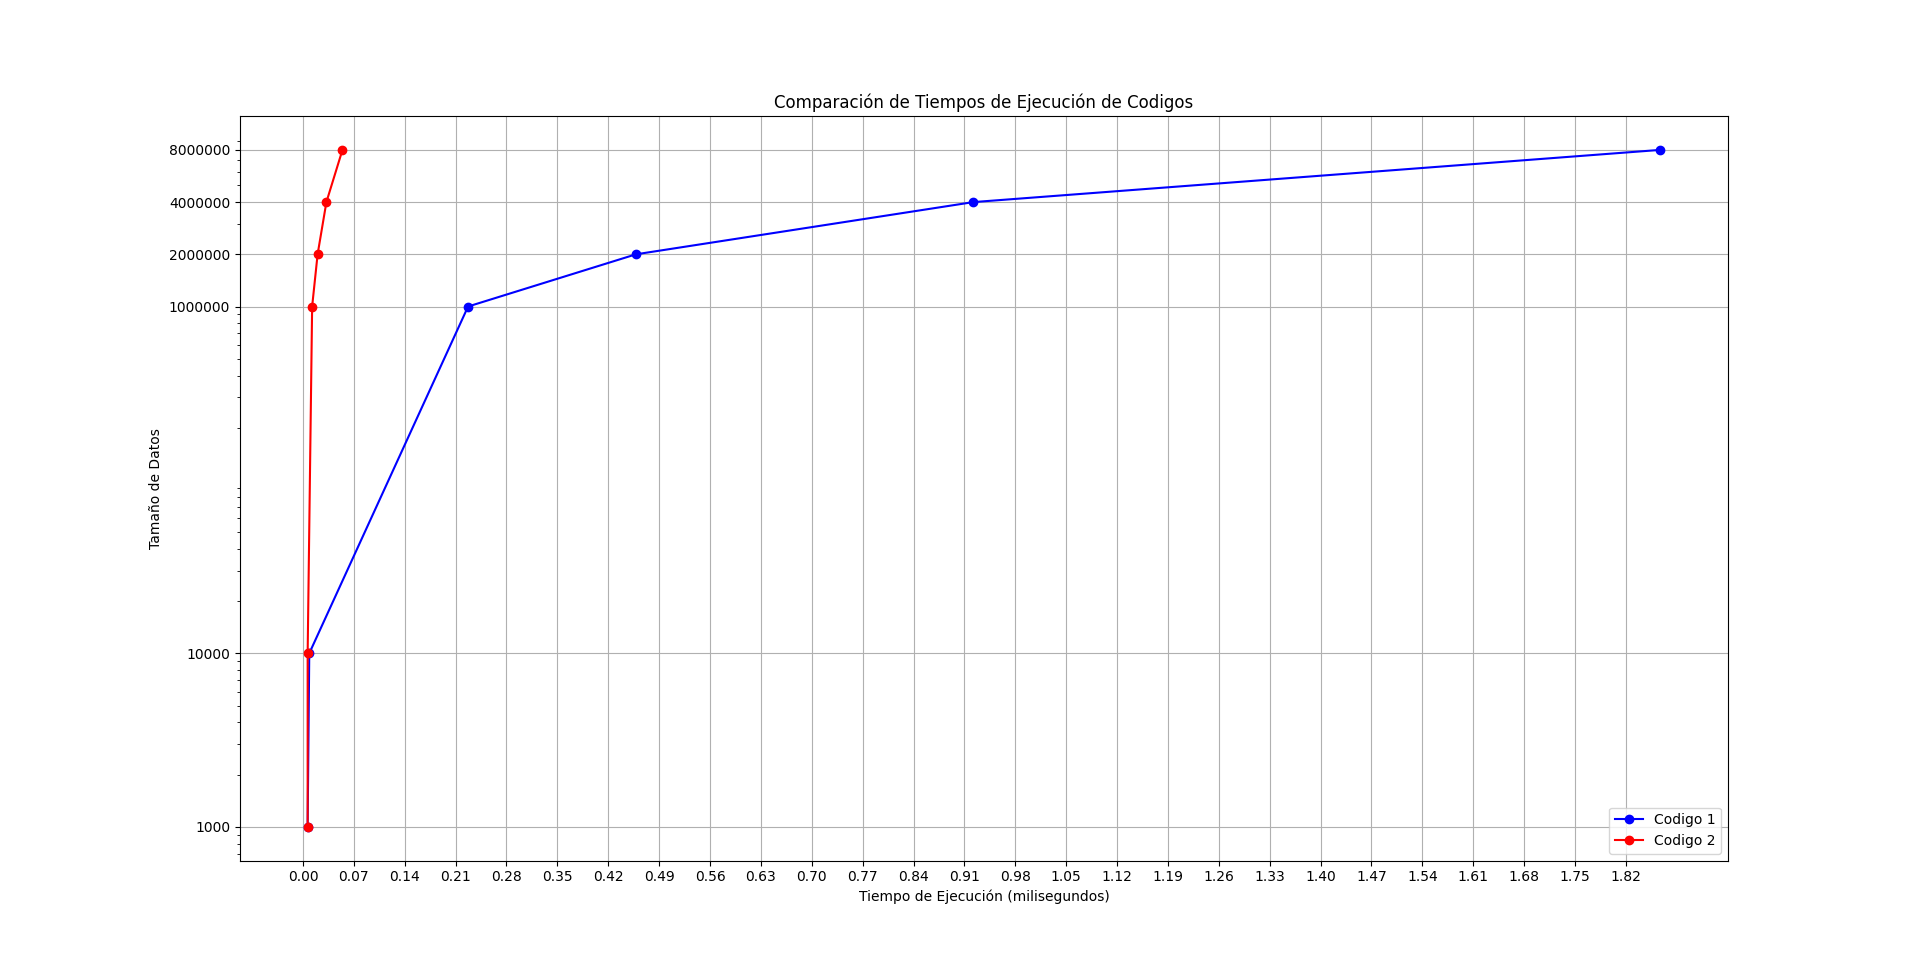
\includegraphics[scale=0.35]{img/mean_times.png}
  \caption{Tiempo promedio de ejecución}
  \label{fig:tiempo promedio de ejecución}
\end{figure}

\begin{table}[H]
  \centering
  \begin{tabular}{|c|c|c|}
    \hline
    \textbf{Tamaño de datos} & \textbf{Tiempo Código 1} & \textbf{Tiempo Código 2} \\ \hline
    1000 & 0.00642909 & 0.00644173 \\ \hline
    10000 & 0.00865969 & 0.00644241 \\ \hline
    1000000 & 0.227177 & 0.0126207 \\ \hline
    2000000 & 0.458186 & 0.0201534 \\ \hline
    4000000 & 0.922377 & 0.0322431 \\ \hline
    8000000 & 1.86746 & 0.0543328 \\ \hline
  \end{tabular}
  \caption{Tiempo promedio de ejecución}
  \label{tab:tiempo promedio de ejecución}
\end{table}

\section{Tiempos máximo de ejecución}
\begin{figure}[H]
  \centering
  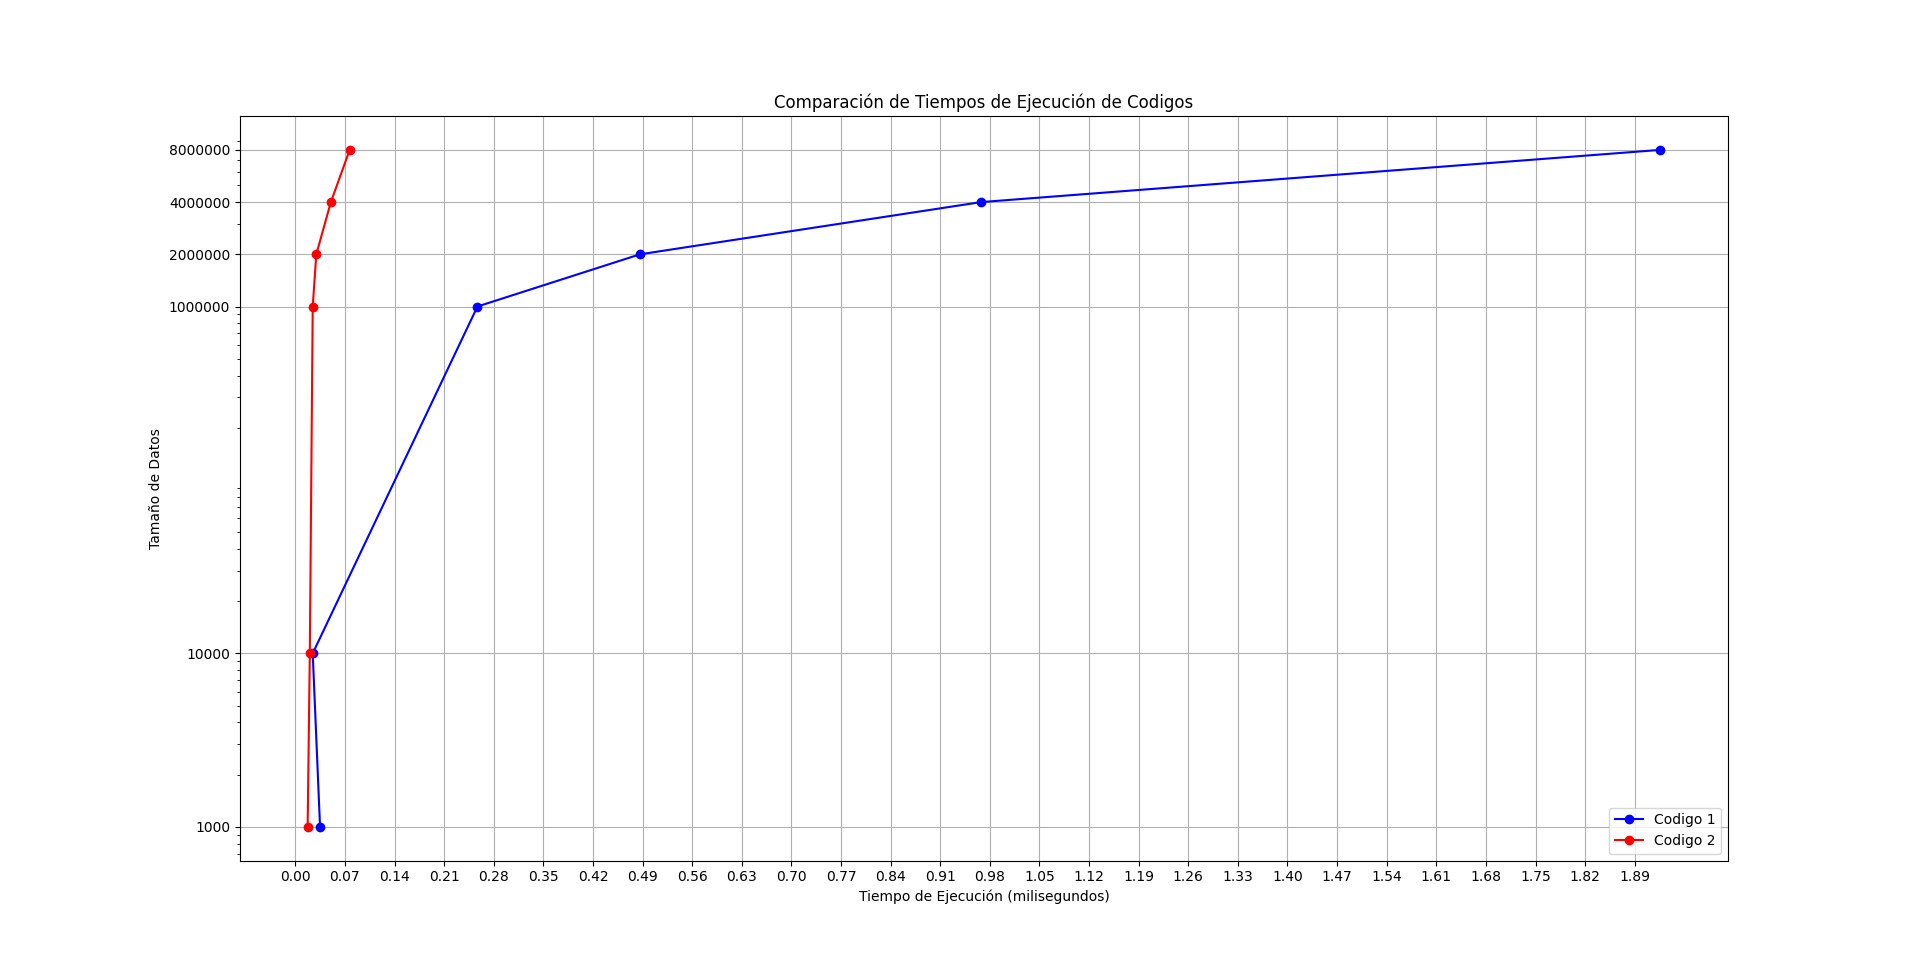
\includegraphics[scale=0.35]{img/max_times.png}
  \caption{Tiempo máximo de ejecución}
  \label{fig:tiempo máximo de ejecución}
\end{figure}

\begin{table}[H]
  \centering
  \begin{tabular}{|c|c|c|}
    \hline
    \textbf{Tamaño de datos} & \textbf{Tiempo Código 1} & \textbf{Tiempo Código 2} \\ \hline
    1000 & 0.034912 & 0.017408 \\ \hline
    10000 & 0.024576 & 0.02048 \\ \hline
    1000000 & 0.257024 & 0.024576 \\ \hline
    2000000 & 0.4864 & 0.029664 \\ \hline
    4000000 & 0.96768 & 0.050176 \\ \hline
    8000000 & 1.92614 & 0.076736 \\ \hline
  \end{tabular}
  \caption{Tiempo máximo de ejecución}
  \label{tab:tiempo máximo de ejecución}
\end{table}

\section{Tiempos mínimo de ejecución}
\begin{figure}[H]
  \centering
  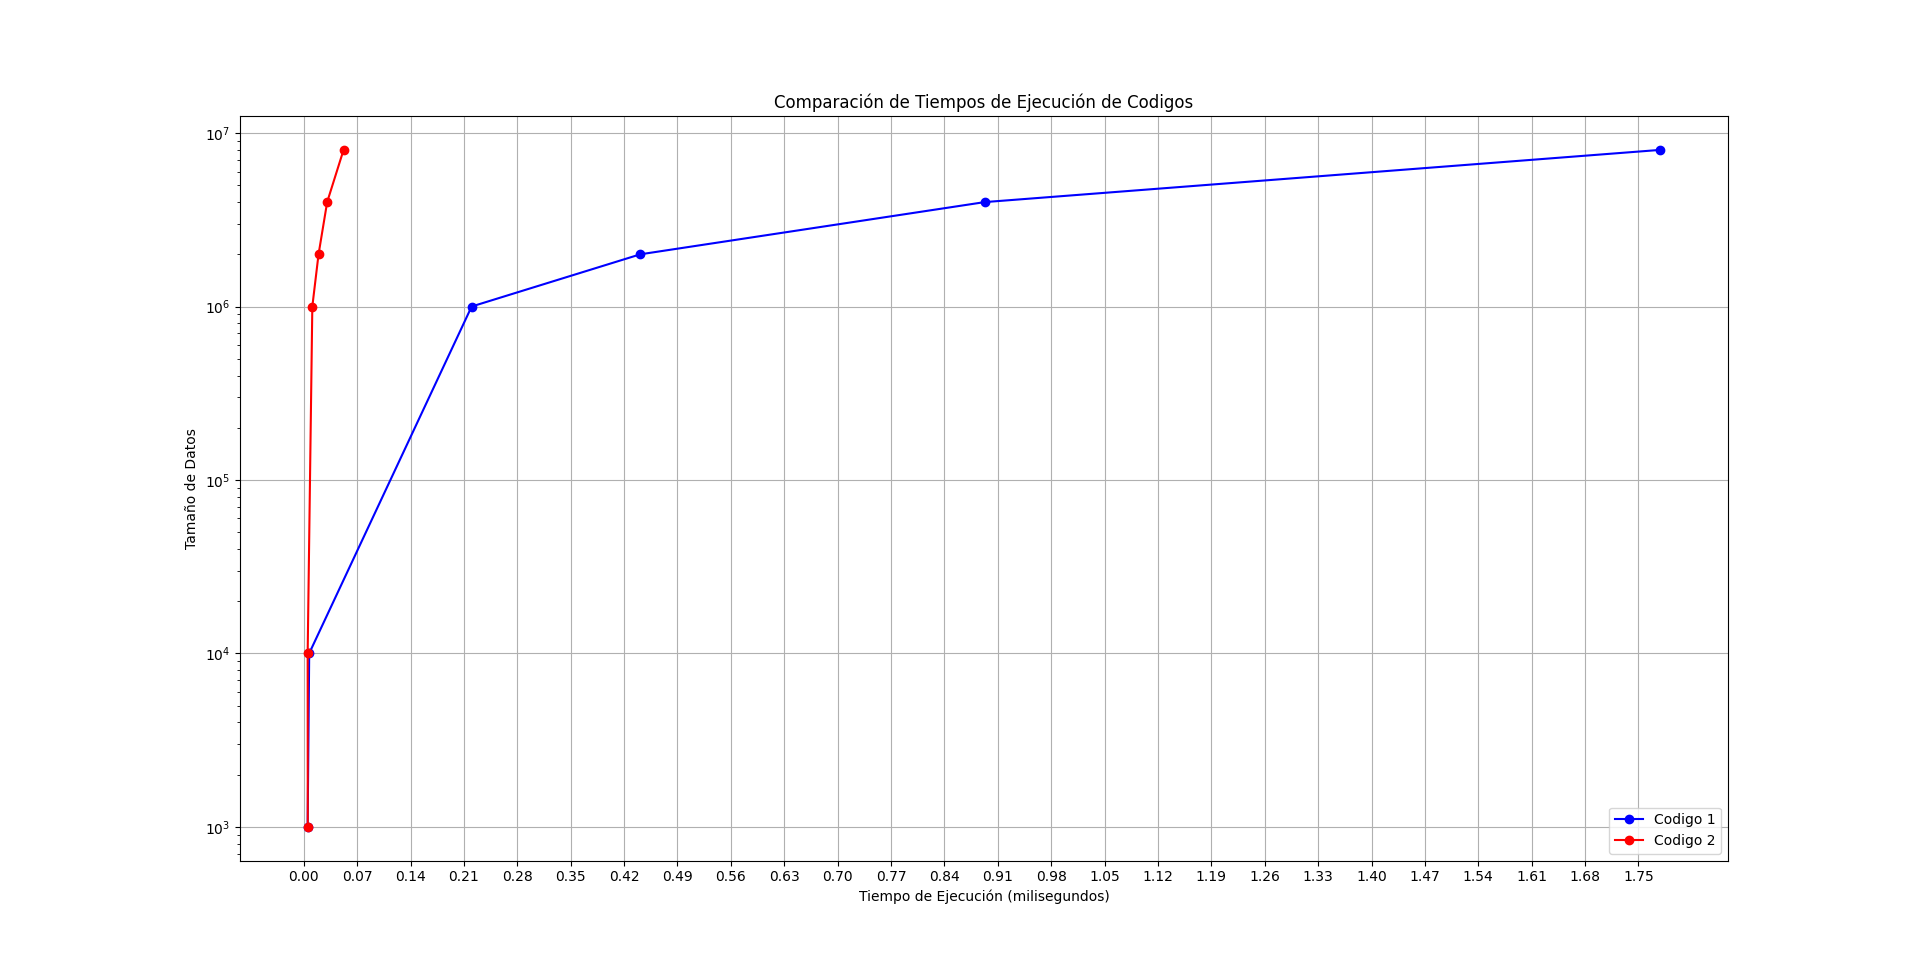
\includegraphics[scale=0.35]{img/min_times.png}
  \caption{Tiempo mínimo de ejecución}
  \label{fig:tiempo mínimo de ejecución}
\end{figure}

\begin{table}[H]
  \centering
  \begin{tabular}{|c|c|c|}
    \hline
    \textbf{Tamaño de datos} & \textbf{Tiempo Código 1} & \textbf{Tiempo Código 2} \\ \hline
    1000 & 0.00512 & 0.00528 \\ \hline
    10000 & 0.007168 & 0.005152 \\ \hline
    1000000 & 0.22016 & 0.011264 \\ \hline
    2000000 & 0.441344 & 0.019424 \\ \hline
    4000000 & 0.892928 & 0.03072 \\ \hline
    8000000 & 1.77869 & 0.052224 \\ \hline
  \end{tabular}
  \caption{Tiempo mínimo de ejecución}
  \label{tab:tiempo mínimo de ejecución}
\end{table}

% Capitulo 4
\chapter{Conclusiones}
En conclusión, la segunda implementación es más eficiente, en comparación con la primera implementación,
debido a que se divide en dos fases. En la primera de ellas, se calcula un histograma local para
cada hilo. Mientras que en la segunda, se realiza la suma de los histogramas locales en un único
histograma global final. Por consecuencia, la primera implementación es menos eficiente, debido a que se utiliza
un único histograma compartido por todos los hilos. 

Además, se ha podido observar que el tiempo de ejecución de la primera implementación es mayor
que el tiempo de ejecución de la segunda. Donde en la primera, el
tiempo de ejecución aumenta de forma exponencial a medida que el tamaño de datos aumenta.
En comparación con la segunda implementación, donde el tiempo de ejecución aumenta de forma lineal a medida que
el tamaño de datos aumenta.

\end{document}